\chapter{Diseño e implementación\label{05disenoTrabajo}}

El proyecto, como ya se comentó en la aplicación está desarrollado principalmente con NodeJS sirviéndose del framework Express, dicha elección tuvo relevancia frente al uso de Python con el framework express dada la buena integración del lenguaje Javascript con el formato JSON, y la facilidad que ofrece para realizar peticiones a un API REST que proporciona los datos en un formato JSON. En este caso, todos los datos de los repositorios, deben ser recuperados a través del proveedor de servicios Git, en este caso GitHub.

GitHub ofrece un completo API REST mediante el cual se puede realizar un control total de la herramienta Git sobre la cuenta de un usuario. Para ello, es necesario ofrecer un token de acceso, el cual se puede solicitar a través de la misma página web de GitHub y el cual es necesario para el funcionamiento y el acceso a los datos de los repositorios por parte de la aplicación desarrollada.

Como veremos en más detalle a continuación, la arquitectura de la aplicación se conforma con dos servidores implementados con NodeJS utilizando el framework Express, y una base de datos para ofrecer persistencia, en este caso una implementación de MySQL.




\section{Arquitectura base de la aplicación.}
En primer lugar, contamos con el servidor web, implementado con NodeJS-Express, este se encargará de servir las peticiones de los usuarios a la página principal de la aplicación web. Implementando en esta todo la interfaz para el usuario, donde se podrá realizar tanto login como usuarios, y donde se visualizará todo el panel de repositorios, asignaturas, y estadísticas.

Dicho servidor, necesita ofrecer persistencia, tanto para el registro de los usuarios, en este caso el profesorado,  como para el posterior inicio de sesión en la aplicación. Además, tanto las asignaturas que los profesores puedan crear, y los repositorios que manualmente pueden añadir a dichas asignaturas deben ser persistidas sobre una base de datos para su persistencia.
Para ofrecer dicha persistencia, se hace uso de una implementación de MySQL, debido a la fácil integración de los datos a persistir con el modelo relacional, con una estructura basada en tablas. Para la integración del servidor web, con la base de datos, se utiliza la librería mysql, ofrecida de manera oficial por el la misma. A través de la misma, podremos mantener y actualizar la información procedente de las acciones de los usuarios en la página web.

Mediante la implementación del servidor web y el servicio de persistencia, podríamos obtener una solución viable y funcional, sin embargo, es conveniente, en este caso, separar el servidor web de la consulta de datos al servicio de GitHub. El servidor web está destinado al múltiple acceso de los usuarios, sobre el cual requerimos de un buen rendimiento y tiempo de respuesta, lo que puede verse afectado por la gestión de múltiples peticiones a otro servicio.

Por consiguiente, se ha implementado un segundo servidor, también desarrollado en NodeJS, el cual está encargado de realizar toda la comunicación con los servidores de Github, es decir, se encargará de obtener toda la información necesaria de los servicios de GitHub. De esta forma, contaremos con:
\begin{itemize}
  \item \textbf{El primer servidor,}servidor web, el cual implementa todo el servicio web, destinado únicamente a recibir y responder las peticiones web de los usuarios. Este servidor será por tanto el encargado de comunicarse con la base de datos y gestionarla, realizando las consultas de registro y creación de usuarios, así como gestionar las asignaturas. En caso de necesitar datos provenientes del API Rest de Github, estos datos se solicitan al segundo servidor.
  \item \textbf{El segundo servidor,}, servidor proxy Rest sobre GitHub, implementa un servicio encargado de atender las peticiones del primer servidor e intercomunicarse con el API de GithuB para obtener los datos solicitados. Por tanto, actúa a modo de proxy para el servicio de GitHub.


\end{itemize}

\begin{figure}[h!]
  \centerline{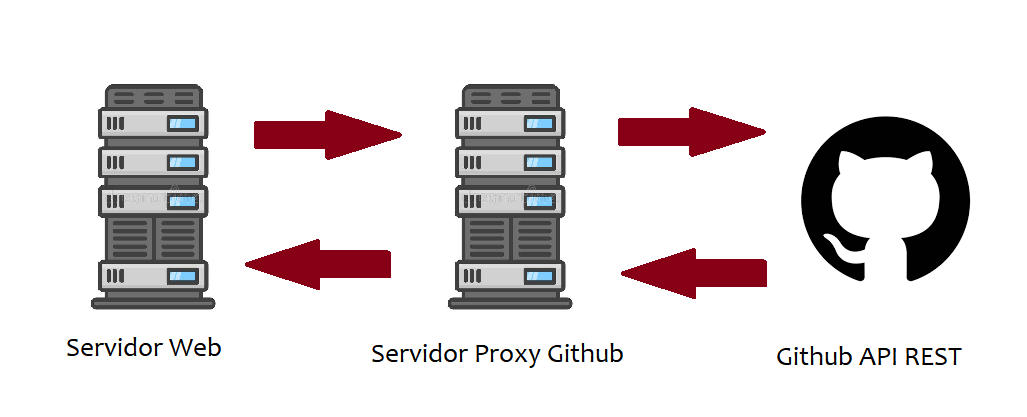
\includegraphics[width=1\textwidth]{Servidores.png}}
  \caption{Grafico de funcionamiento de los servidores implementados y el servicio API de GitHub.}
  \label{figure:servidores}
\end{figure}
En la figura~~\ref{figure:servidores}, se representa mediante un gráfico el flujo de comunicación entre los servidores implementados y el API que ofrece GitHub.

Respecto la comunicación de los dos servidores, el segundo servidor está implementado a modo de API REST, donde recibe peticiones HTTP, en este caso únicamente recibe peticiones de tipo Get, recibiendo por los parámetros de la url los datos que se desean obtener, vez recibida la petición y procesada, se comunica con el API de GIthub, obtiene los datos correspondientes y responde de nuevo al primer servidor.

\begin{figure}[h!]
  \centerline{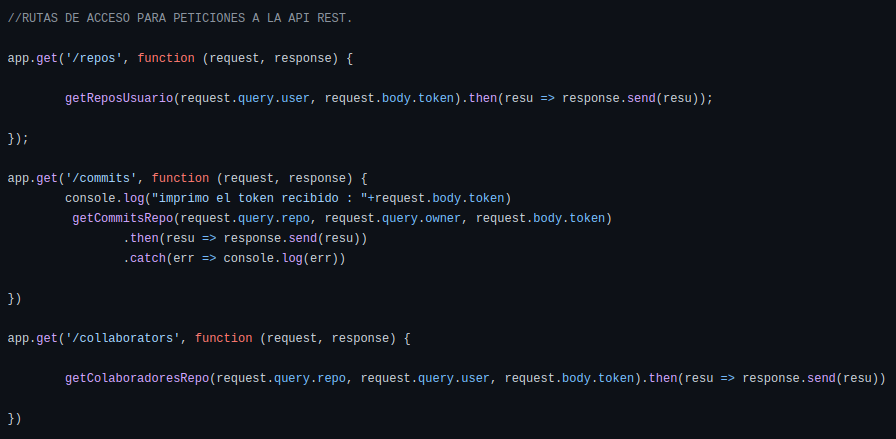
\includegraphics[width=1\textwidth]{ProxyGitHub.png}}
  \caption{Configuración del servidor proxy GitHub, implementación en NodeJS con Express.}
  \label{figure:ProxyGitHub}
\end{figure}
En la figura~~\ref{figure:ProxyGitHub}, se muestran los diferentes metodos get y la forma de especificar que información se desea recuperar mediante el uso de parametros en la url de la petición.


Como hemos comentado, las causas de la implementación del segundo servidor, es destinar únicamente el servidor web para los usuarios y no sobrecargarlo con peticiones a otro servicio externo, reduciendo así su carga de trabajo y mejorando los tiempos de respuesta. Además, conseguimos de esta forma, separar la arquitectura de la aplicación, teniendo por una parte la implementación del frontend, a la cual tienen acceso los clientes , y el backend, encargado de proveer la información al frontend, de tal forma que ambos servicios son independientes y obteniendo un buen rendimiento en ambos, en aquellos casos en los que puedan ocurrir múltiples peticiones. Posteriormente, veremos esta separación, también permite distribuir mejor la aplicación desarrollada sobre un servicio cloud, permitiendo escalar cada servicio en medida de la sobrecarga que se produzca.



\section{Consulta de datos al API de GitHub y autenticación.}

Para la implementación de la aplicación, se utiliza la librería “Octokit”, una librería ofrecida de forma oficial por el proveedor de servicios, y cual se integra con el lenguaje javascript, mediante ella, podemos realizar las consultas al API de Github de una manera sencilla y teniendo acceso a operaciones que requieren acceso mediante token. Con esta librería, las peticiones realizadas, se configuran con las cabeceras adecuadas para garantizar la seguridad necesaria.Vemos a continuación, un fragmento de código que representa en javascript la obtención de una instancia de la librería y una función utilizada para recuperar la información de un usuario a través del API proporcionada.

\begin{figure}[h!]
  \centerline{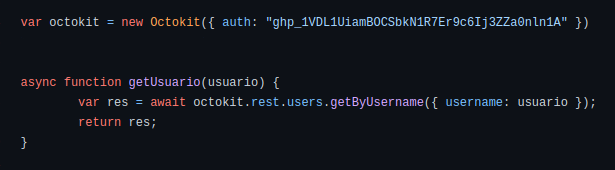
\includegraphics[width=1\textwidth]{octokit.png}}
  \caption{Ejemplo de uso de la librería Ocktokit, ofrecida por GitHub.}
  \label{figure:octokit}
\end{figure}

En la figura~~\ref{figure:octokit}, se muestra la creación e inicialización de un objeto “Octokit”, objeto ofrecido por la librería, mediante el cual posteriormente se realizarán las peticiones HTTP, para su creación le brindamos el token del usuario, necesario para poder leer la información de sus repositorios. 



\section{Maquetado de la aplicación web.}

La funcionalidad de la web debe ser, en un primer lugar, permitir registro e inicio de sesión. Y en segundo lugar, mostrar los repositorios, permitiendo el filtrado o bien por cadenas de caracteres, o bien por filtrado en base a asignaturas previamente creadas por el usuario de la sesión.

Para la implementación de la web, se basa en cuatro vistas diferentes, dos de ellas para registro e inicio de sesión, una para la página de inicio, donde se muestran los repositorios y asignaturas del usuario, y por último la página donde se visualizan las estadísticas del repositorio, esta última accesible al hacer click sobre algún repositorio en la página principal.

Para el diseño de las vistas, se ha utilizado tecnologías específicas para la tarea, dando estructura a las páginas con HTML, para posteriormente añadir con css y bootstrap estilos, y por último implementar animaciones y eventos en javascript.

En el caso de la página de las páginas de inicio de sesión y estadísticas, al solicitar las webs al servidor, este nos envía la estructura y diseño de la web, además del código javascript asociado a la página,  mediante el cual, se solicitarán de manera asíncrona, la información al servidor para completar las vistas. Por ejemplo, en el caso de acceder a la página principal, el servidor nos responde con una tabla vacía, que justo cuando se recibe, se realiza otra petición asíncrona al servidor que una vez resuelta, hará que los datos se muestren en el interior de la tabla. 

Para ello, implementamos mediante javascript funciones que se ejecutarán una vez la página se haya cargado en el navegador que realicen el completado de la vista con la información obtenida. De esta forma, logramos que la respuesta a la petición sea inmediata, y posteriormente cuando los datos sean recuperados se muestran, así, el usuario no percibe un retraso al acceder al sitio web, como ocurriría si esperamos a enviar la web desde el servidor una vez los datos de GitHub se hayan recuperado.


\section{Contenerización y despliegue de aplicación.}

El segundo objetivo del proyecto, es ofrecer una implementación útil para el despliegue en un servicio cloud, de tal forma que los servicios, estén basados en contenedores, que puedan ser lanzados en una estructura de nodos cloud, permitiendo así su control y escalado. Por consiguiente, se ofrecen junto el proyecto, las herramientas necesarias para formar contenedores con cada uno de los servicios implementados, en primer lugar, una imagen Docker para cada uno de los servidores Node, y un fichero docker-compose como herramienta para simplificar el despliegue, de tanto, ambos servidores en Node, como un contenedor para la base de datos MySQL, configurado e inicializado para funcionar de forma integrada con los otros servicios.

Estos contenedores, en caso de contar con un proveedor cloud, o el hardware correspondiente, se pueden desplegar y escalar, por ejemplo, usando para el propósito un orquestador como podría ser Kubernetes, uno de los gestores de contenedores más popular a día de hoy. Permitiéndonos establecer configuraciones donde podríamos lanzar los servicios y en caso de caída de alguno de ellos levantarse de forma automática. Además, ofrece posibilidades como el escalado automático en momentos donde la carga de trabajo está creciendo de manera paulatina, repartiendo así la carga de trabajo y evitando el colapso.

En caso de querer realizar un despliegue normal, bien sea, en un ordenador personal o en un servidor, se ofrecen dos alternativas de despliegue:

  \begin{enumerate}
    \item Desplegar los servidores de manera manual, iniciándose mediante consola. Usando para ello los comandos:

          \begin{itemize}
            \item \textit{“npm install“},para instalar las dependencias necesarias, en caso de no estas previamente instaladas.
            \item \textit{“node app.js“}, para lanzar el servidor, quedando en escucha en el puerto 3000.
          \end{itemize}
          Este proceso debemos repetirlo también para el segundo servidor contenido en la carpeta “restjs”, cambiando el segundo comando por “node app2.js”.
    
          Con esto lanzaremos ambos servidores, pero tendríamos que tener instalada y configurada una instancia de MySQL, la cual podríamos inicializar utilizando el fichero “schema.sql” situado en la carpeta “scripts”.
    
     \item La segunda opción, por otro lado, sería utilizar el Docker-compose ofrecido junto el proyecto, para el cual únicamente deberíamos ejecutar “docker compose up”.
     
          Este comando se encargaría de construir las imágenes de ambos servidores, recuperar una imagen oficial de MySQL desde el repositorio Docker Hub, configurar los volúmenes necesarios, y crear y configurar la subred necesaria para la intercomunicación de los mismos.
     

  \end{enumerate}

\begin{lstlisting}
version: '2'

services:
  nodejs:
    build:
      context: .
      dockerfile: Dockerfile
    image: nodejs
    container_name: nodejs
    restart: unless-stopped
    environment:
      - MYSQL_HOST=db
      - PROXY_REST=restjs
    ports:
      - "3000:3000"
    volumes:
      - .:/home/node/app
  
  restjs:
    build: ./restjs
    restart: unless-stopped
    ports:
      - "3001:3001"
    volumes:
    - .:/home/node/restjs 
    expose:
      # Opens port 3001 on the container
      - '3001'  
   

  db:
    image: mysql
    restart: always
    command: --default-authentication-plugin=mysql_native_password
    environment:
      MYSQL_DATABASE: 'nodelogin'
      # So you don't have to use root, but you can if you like
      MYSQL_USER: 'user'
      # You can use whatever password you like
      MYSQL_PASSWORD: 'root'
      # Password for root access
      MYSQL_ROOT_PASSWORD: 'root'
    ports:
      # <Port exposed> : < MySQL Port running inside container>
      - '3005:3306'
    expose:
      # Opens port 3306 on the container
      - '3005'
      # Where our data will be persisted
    
    volumes:
      - "./scripts/schema.sql:/docker-entrypoint-initdb.d/1.sql"

\end{lstlisting}

Vemos la configuración del .yml construido para el arranque de los servicios mediante Docker-Compose, es de destacar, la configuración de los servicios, introduciendo como variables de entorno los nombres asignados, de esta forma se resuelve el direccionamiento de forma automática, mediante una subred que crea Docker-Compose y mediante dichas variables posteriormente en el programa podemos acceder al resto de servicios configurados. Además, destacamos la configuración de los volúmenes, y la inicialización de la base de datos, para contruir el schema con un fichero de inicialización para MySQL.
%%% Local variables:
%%% TeX-master: "memoria.tex"
%%% coding: utf-8
%%% ispell-local-dictionary: "spanish"
%%% TeX-parse-self: t
%%% TeX-auto-save: t
%%% fill-column: 75
%%% End:

%  LocalWords:  NoSQL schemaless metadatos
